\documentclass[10pt]{article}
\usepackage[usenames]{color} %used for font color
\usepackage{amssymb} %maths
\usepackage{amsmath} %maths
\usepackage[utf8]{inputenc} %useful to type directly diacritic characters
\usepackage{tikz}
\usetikzlibrary{arrows,positioning,decorations.pathreplacing} 

\definecolor{boiseBlue} {RGB}{29,72,159}
\definecolor{rojoAmor} {RGB}{171,13,4}
\definecolor{moradoAmor} {RGB}{93,8,113}
\definecolor{verdeAmor} {RGB}{98,158,31}
\definecolor{negro} {RGB}{10,10,10}
\definecolor{lgreen} {RGB}{180,210,100}
\definecolor{dblue}  {RGB}{20,66,129}
\definecolor{ddblue} {RGB}{11,36,69}
\definecolor{lred}   {RGB}{220,0,0}
\definecolor{nred}   {RGB}{224,0,0}
\definecolor{norange}{RGB}{230,120,20}
\definecolor{nyellow}{RGB}{255,221,0}
\definecolor{ngreen} {RGB}{98,158,31}
\definecolor{dgreen} {RGB}{78,138,21}
\definecolor{nblue}  {RGB}{28,130,185}
\definecolor{jblue}  {RGB}{20,50,100}\begin{document}
\[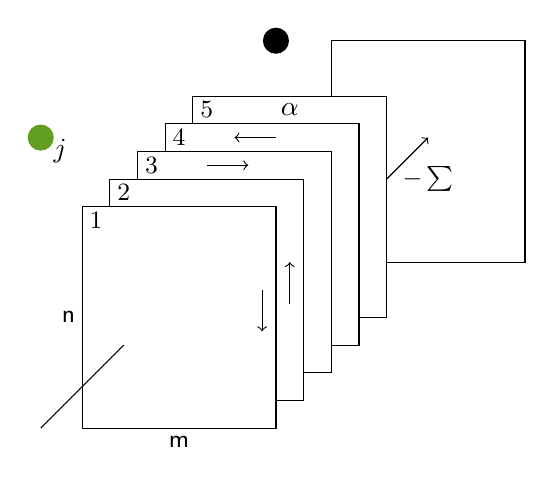
\begin{tikzpicture}
%
\node[draw=black,minimum width=7em,minimum height=8em,rectangle,fill=white]  at (9em,6em) {};
\node[draw=black,minimum width=7em,minimum height=8em,rectangle,fill=white]  at (4em,4em) {};
\node[draw=black,minimum width=7em,minimum height=8em,rectangle,fill=white]  at (3em,3em) {};
\node[draw=black,minimum width=7em,minimum height=8em,rectangle,fill=white]  at (2em,2em) {};
\node[draw=black,minimum width=7em,minimum height=8em,rectangle,fill=white]  at (1em,1em) {};
\node[draw=black,minimum width=7em,minimum height=8em,rectangle,fill=white]  at (0,0) {};
%
\node[fill=ngreen,circle]  at (-5em,6.5em) {};
\node[fill=black,circle]  at (3.5em,10em) {};
%\node[]  at (-5em,6.5em) {$\varphi_i$};
\node[]  at (-4.3em,6em) {$\small{j}$};
%
\node[]  at (-3em,3.5em) {\small{1}};
\draw[->] (1em,5.5em) -- (2.5em,5.5em);
\node[]  at (-2em,4.5em) {\small{2}};
\draw[<-] (2em,6.5em) -- (3.5em,6.5em);
\node[]  at (-1em,5.5em) {\small{3}};
\draw[<-] (3em,-0.5em) -- (3em,1em);
\node[]  at (0em,6.5em) {\small{4}};
\draw[->] (4em,0.5em) -- (4em,2em);
\node[]  at (1em,7.5em) {\small{5}};
\node[]  at (4em,7.5em) {$\small{\alpha}$};
%
\draw[->] (7.5em,5em) -- (9em,6.5em);
\node[]  at (9em,5em) {\small{$-\sum$}};
\draw[-] (-5em,-4em) -- (-2em,-1em);
%
\node[]  at (-4em,0em) {\small{\sf n}};
\node[]  at (0em,-4.5em) {\small{\sf m}};
\end{tikzpicture}
\]
\end{document}